% Chapter 1

\chapter{Provenance in the Application's Context} % Write in your own chapter title
\label{Provenance in the Application Context}
\lhead{Chapter 4. \emph{Provenance in the Application Context}} % Write in your own chapter title to set the page header

\section{introduction}

In the previous section we have extensively covered the concept of provenance of electronic data. We went through the benefits of capturing provenance information. We then presented different data models for representing, as well as, locating and retrieving that information. The purpose of this chapter is to describe all those concepts, in the scope of the web application that we developed. We will start by reviewing the benefits that provenance brought to our application. Then the data for which provenance is tracked, will be presented. Finally, we briefly describe how the application stores and exposes that information to external applications.

\section{Benefits of Provenance}

Our web application is a provenance-aware crowd sourced system for monitoring GHG emissions caused by commuter travels. In essence, users are the main source of information; they insert some data pertaining to the travels they make and the application calculates the GHG emissions they produce. It is critical for users to be able to verify the correctness of such calculations. To make that possible, the application needs to track all the steps in the carbon emissions calculation process: the module responsible for calculating carbon emissions has to compile all emissions sources for the subject (in the context of this application, emission sources refer to the trip made by users). Then, an appropriate method for quantifying the emissions of each source has to be selected. Finally, the data required by the method should be gathered, so that carbon emissions for the trip in question can be computed.
In order to verify and validate the computed figure, one should be able to view details for each of those steps; for instance, consider that the total amount of carbon emissions of an individual needs to be verified. In that case, the emission sources that were used have to be presented. Further, the calculation methods, as well as, the data used (i.e. activity data and emission factors), need to be examined.
It is obvious that all the aforementioned data are already stored in the applications' persistence storage (i.e. database). However, what is missing are the connections (dependencies) between those data. This gap is filled by implementing a software component responsible for provenance related tasks. What follows is a descriptions of those tasks.

\section{Tracking Provenance}

In this section we will explain how our application captures, stores and exposes provenance information. We start by presenting the provenance graphs that represent that information.

\subsection{Trip Creation Process}

One of the chief functionalities provided by the application is the insertion of trips. Users, add with the aid of an interactive web UI (refer to chapter 5 for more details) the trips that they make.
The provenance manager, which is the system's component responsible for provenance-related tasks, creates a provenance graph during the process of creating new trips (the "trip creation" process). Figure \ref{fig:provTripCreationGraph}, illustrates a visualized form of that graph, which reveals the provenance of a trip made by the user.

\begin{figure}[htbp]
	\centering
		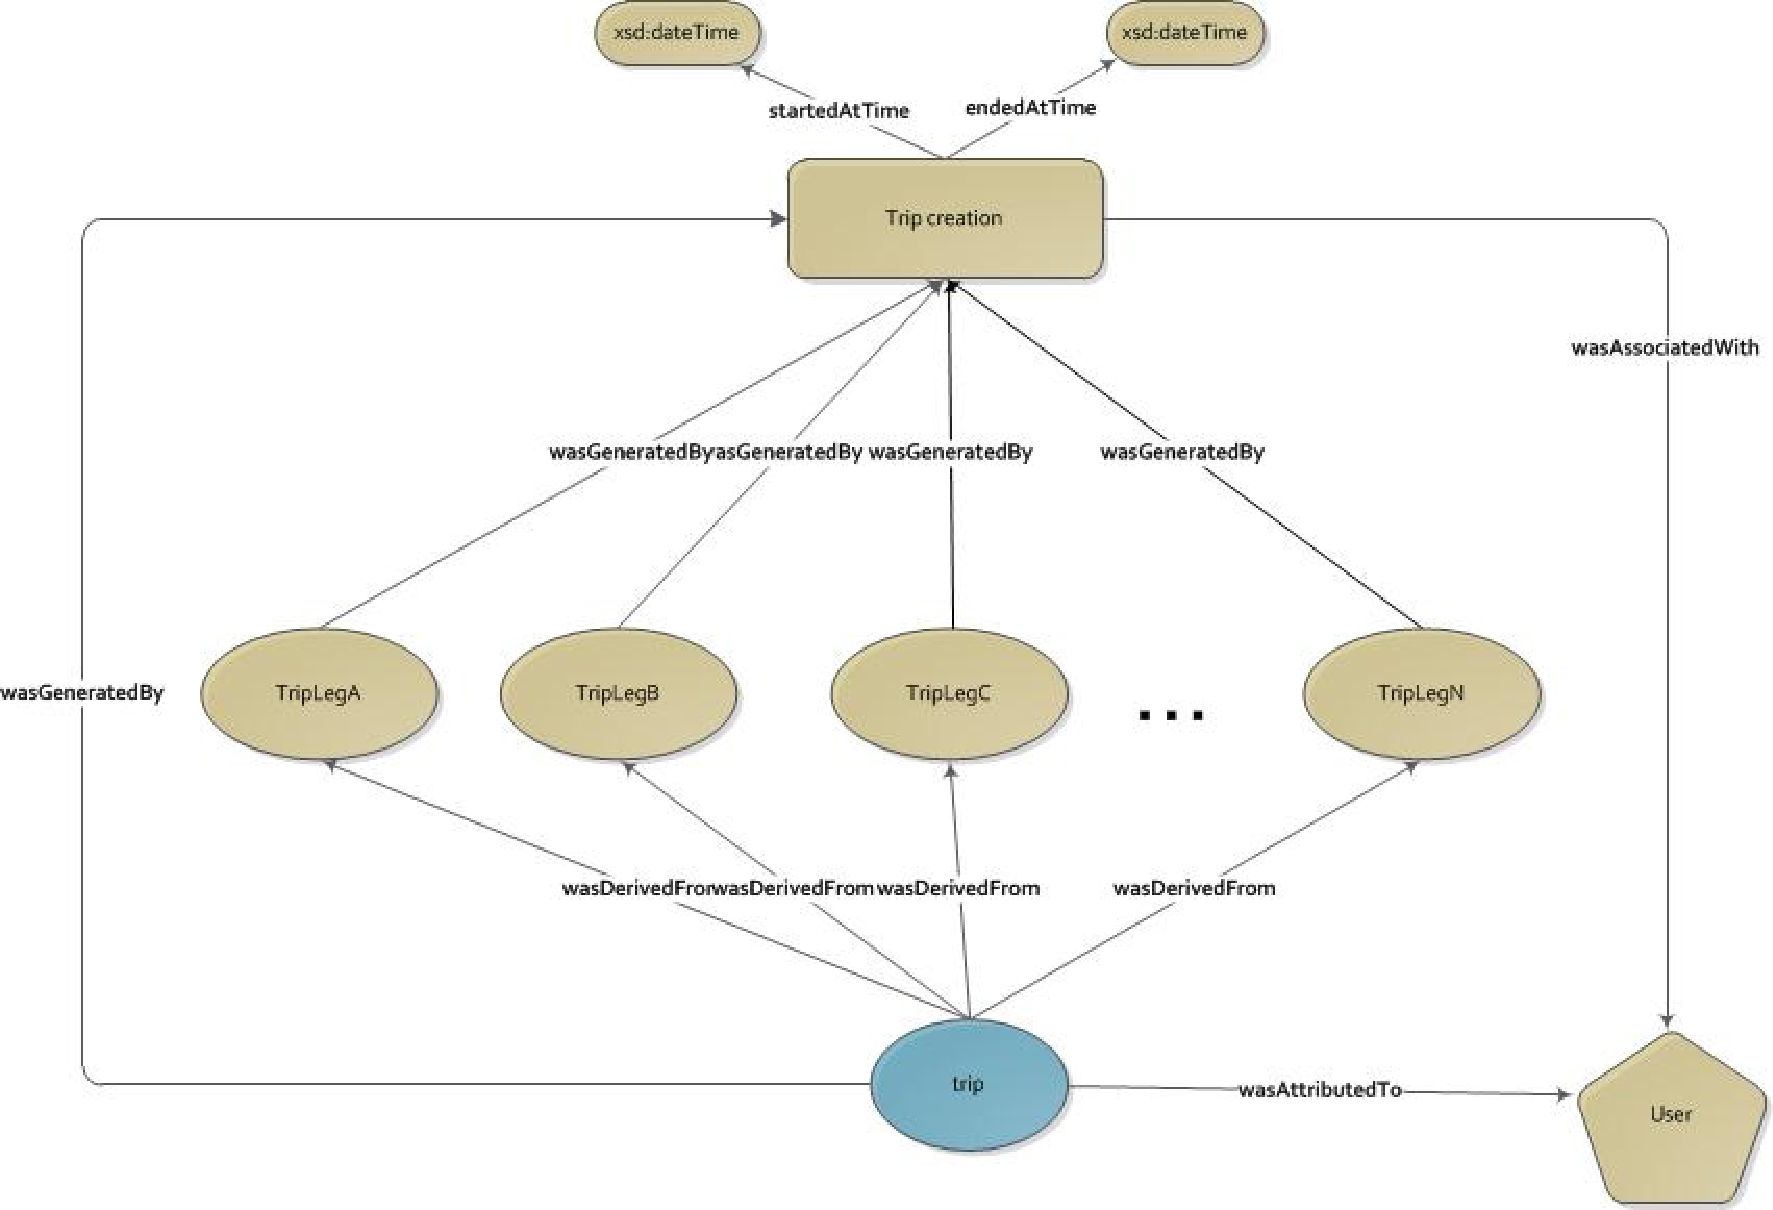
\includegraphics[scale=0.60]{./Figures/chapter3/figure1.pdf}
		\rule{35em}{0.5pt}
	\caption[Trip creation provenance graph]{Trip creation provenance graph.}
	\label{fig:provTripCreationGraph}
\end{figure}

The application adopts the PROV-DM model to represent provenance information. For this reason the graph in figure \ref{fig:provTripCreationGraph} consists of entities, activities and agents, as well as, the relationships among them.

The trip entity refers to the trip that was created during the "trip creation" process.  Each trip might consist of several intermediary steps, which we call "trip legs". This is the reason why the \emph{wasDerivedFrom} property connects the trip entity with the corresponding trip legs entities.

Each trip and trip leg is created (\emph{wasGeneratedBy} edge) via the "trip creation" process, which corresponds to the "TripCreation" activity. In some cases it is required to know the computational time of that activity. For this reason the provenance graph includes two additional nodes, storing the start and end time of that activity. Finally users are responsible for creating new trip. Hence, an agent node is added denoting that users has a degree of responsibility for the "Trip Creation" activity.

\subsection{Trip Leg Calculation Process}

During the "Trip creation" process, the system initiates the "Trip Leg Calculation" process. This process, calculates the carbon emissions for each trip leg, based on the data provided by the user. It is the responsibility of this process to select the activity data and an appropriate emission factor (based on the mode of transport used) that will be used in the calculation formula.

The provenance graph that is created during this phase is illustrated in figure \ref{fig:provTripLegCo2Graph}.

\begin{figure}[htbp]
	\centering
		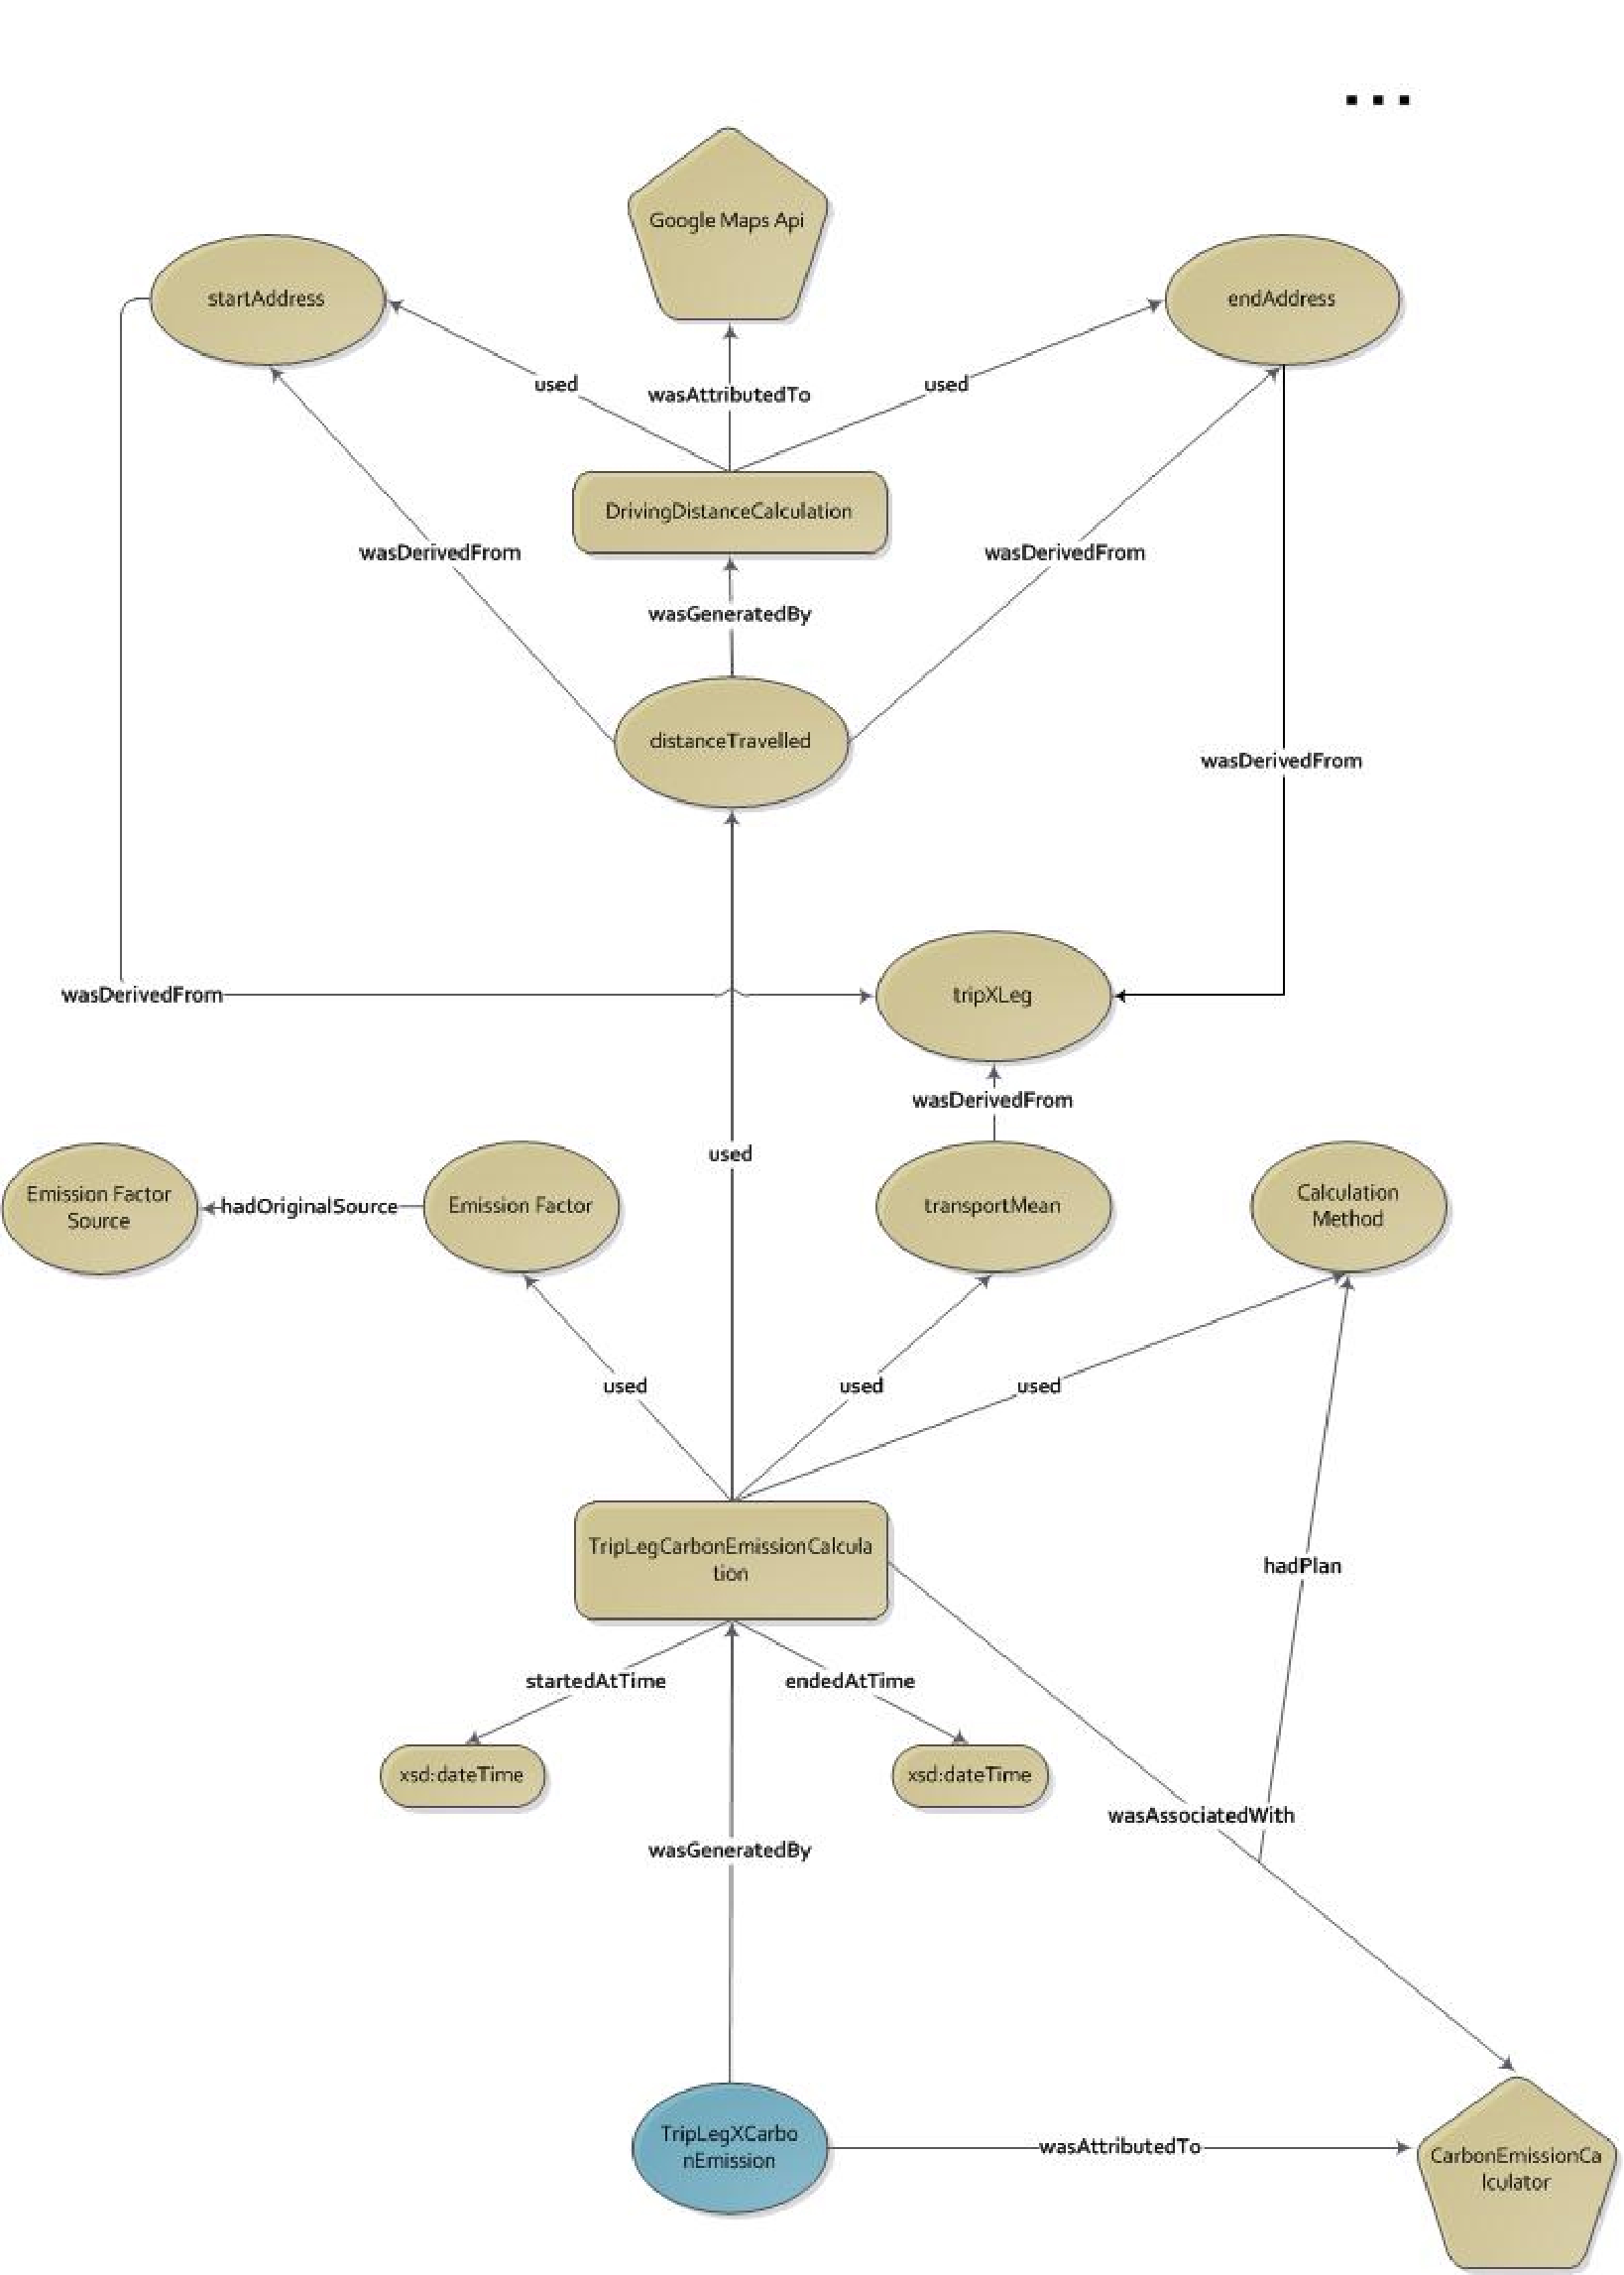
\includegraphics[scale=0.60]{./Figures/chapter3/figure2.pdf}
		\rule{35em}{0.5pt}
	\caption[Graph illustrating the provenance of the TripXLegCarbonEmission entity]{Graph illustrating the provenance of the TripXLegCarbonEmission entity.}
	\label{fig:provTripLegCo2Graph}
\end{figure}

The "TripLegCarbonEmissionsCalculation" activity, which is initiated by the "CarbonEMissionCalculation" agent, corresponds to the process of computing the carbon emissions for a specific trip leg.  The calculation process needs some sort of activity data and appropriate emissions factor, based on the mode of transport used. Ultimately, those data are combined via a calculation method to produce the carbon emissions for that trip leg. The relationship is expressed via the used edges from the "TripLegCarbonEmissionsCalculation".

The "distanceTravelled" entity represents the driving distance travelled by the transport mean. This figure is computed dynamically through a service (DrivingDistanceCalculation) provided by a third party application (GoogleMaps API). The input data for this service are the source and destination addresses of the trip. Finally, there can be several organizations that publish emission factors; we need to explicitly specify the source of the emission factor. For this reason, the \emph{hadPrimarySource} edge from "emissionsFactor" to "emissionFactor Source" is added.


\subsection{Trip Carbon Emissions Calculation Process}

The process of calculating the total carbon emissions caused by a trip is relatively straightforward. It simply sums together the carbon emissions caused by all the intermediary trip legs.

\begin{figure}[htbp]
	\centering
		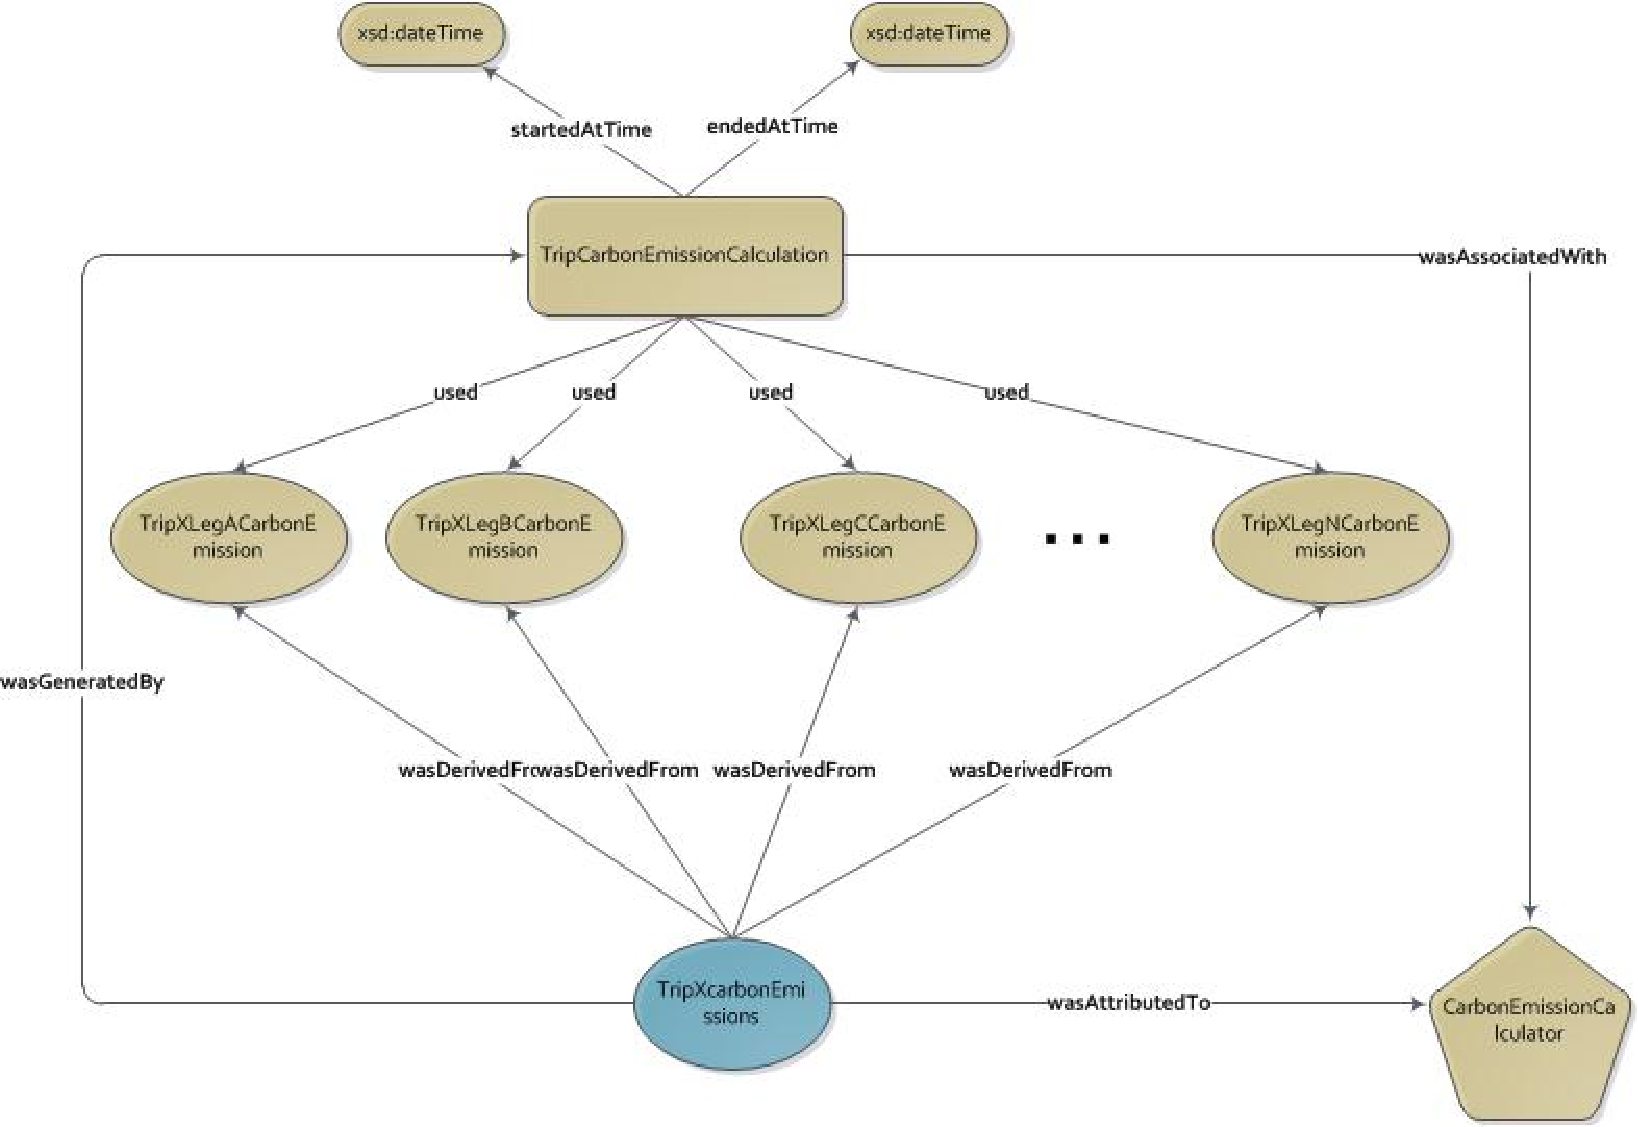
\includegraphics[scale=0.60]{./Figures/chapter3/figure3.pdf}
		\rule{35em}{0.5pt}
	\caption[ Graph illustrating the provenance of the carbon emissions of a trip]{ Graph illustrating the provenance of the carbon emissions of a trip}
	\label{fig:provTripCo2Graph}
\end{figure}

Figure \ref{fig:provTripCo2Graph} demonstrates a graph that describes the provenance the carbon emissions caused by a trip, that is, how that value was derived. The calculation of carbon emissions is processed by the "TripCarbonEmissionCalculation" activity, which sums the the carbon emissions of all the intermediary trip legs to compute that total emissions for the trip (TripXCarbonEMissions).  The dependency is represented via \emph{wasDerivedFrom} edges. Finally, the "CarbonEmisisonCalculator" agent is responsible for undertaking the whole process.

This is good point to demonstrate an example describing how a provenance graph can help users validate their carbon emissions. Consider a scenario where the user modifies the data for one trip leg of a hypothetical trip (TripX). Assume that she changed the transport mean used during that trip leg. At some point, though, she realizes that there is a significant fluctuation between the old and the new value. More specifically, the new carbon emissions value for TripX is much higher than the previous one. In order to verify that there was no error during the calculation process; user can navigate through the provenance of that value (see figure \ref{fig:provTripCo2GraphRevision}).


\begin{figure}[htbp]
	\centering
		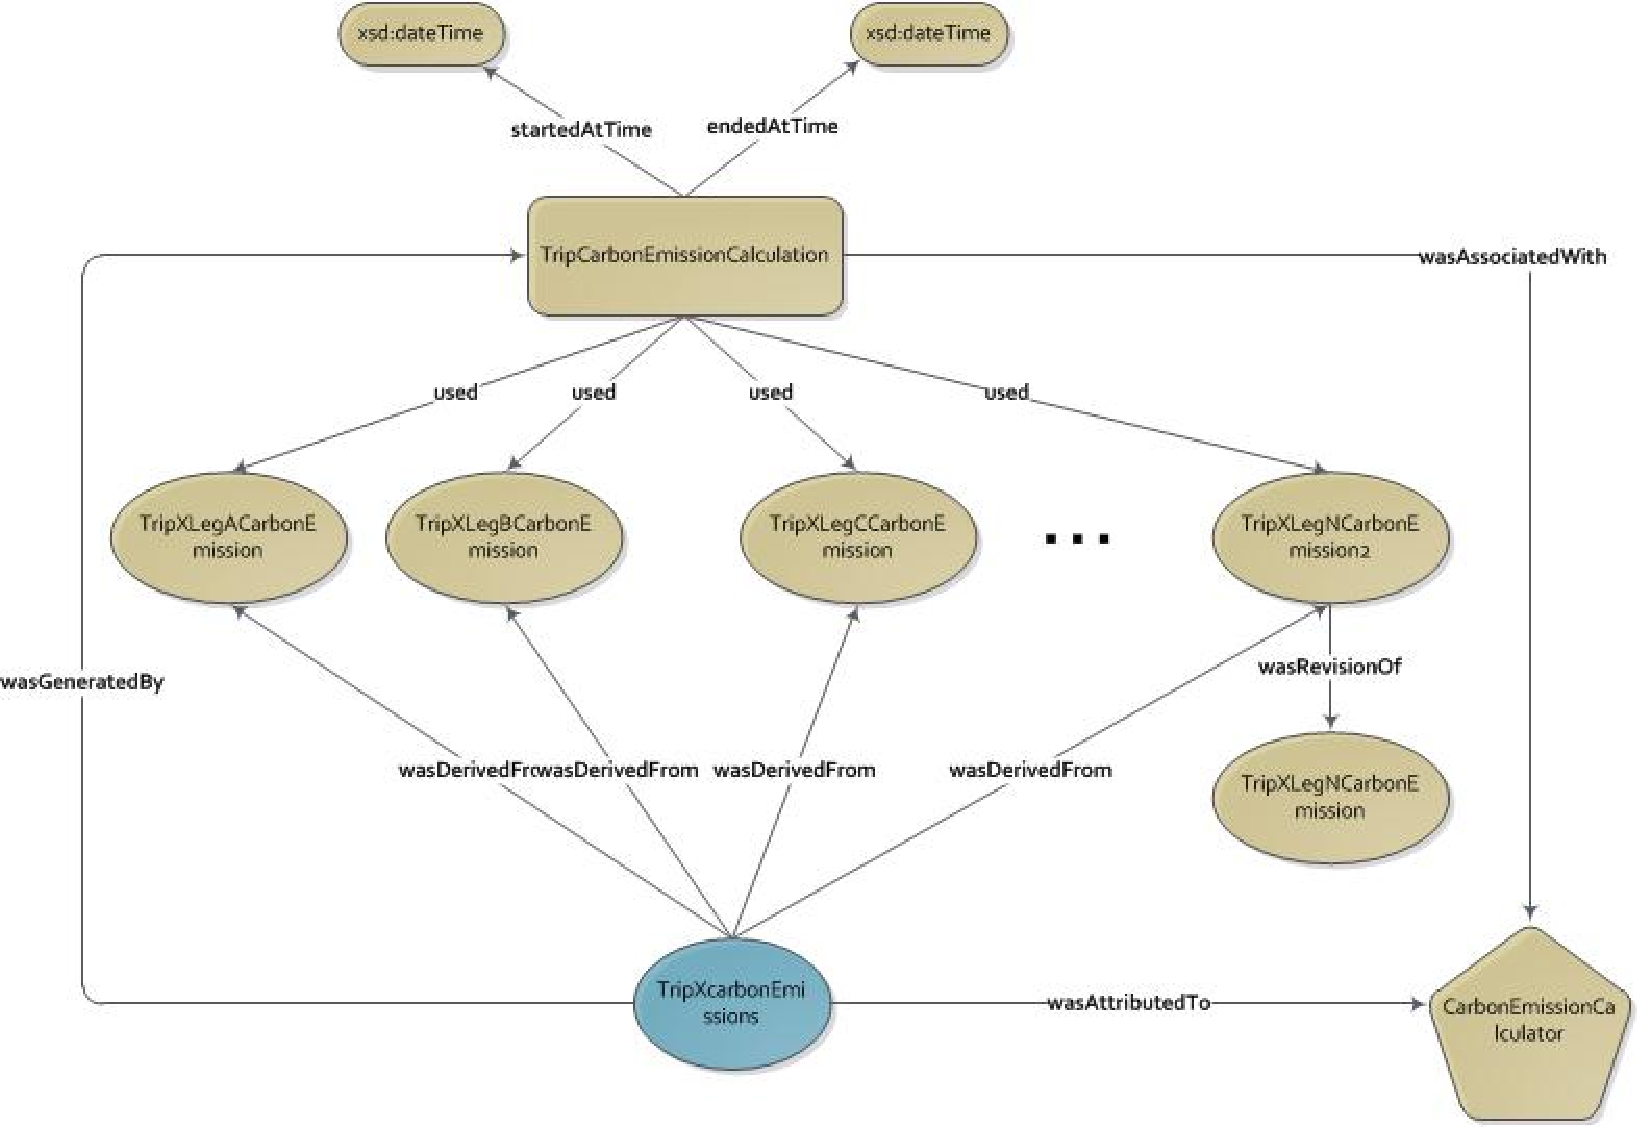
\includegraphics[scale=0.60]{./Figures/chapter3/figure4.pdf}
		\rule{35em}{0.5pt}
	\caption[Graph illustrating the provenance of the carbon emissions of a trip after a trip leg was modified]{Graph illustrating the provenance of the carbon emissions of a trip after a trip leg was modified}
	\label{fig:provTripCo2GraphRevision}
\end{figure}

The graph reveals that the "TripXLegNCarbonEmission" entity has been modified and replaced by the "TripXLegNCarbonEmission2" entity. Ultimately, by investigating the provenance of the new entity (the provenance graph is similar to the one illustrated in figure \ref{fig:provTripLegCo2Graph}), she realizes that she has accidentally inserted the wrong transport mean.

The same approach can be followed when the validation for values for which provenance information is stored, is needed.


\subsection{Calculation process for individual and group carbon emissions}

The application gives a chance for users to view a report where details about individual carbon emissions are presented. One of the information included in that report is the total carbon emissions caused by all the trips made by the user. To achieve that, the carbon emissions for all trips are summed together.

\begin{figure}[htbp]
	\centering
		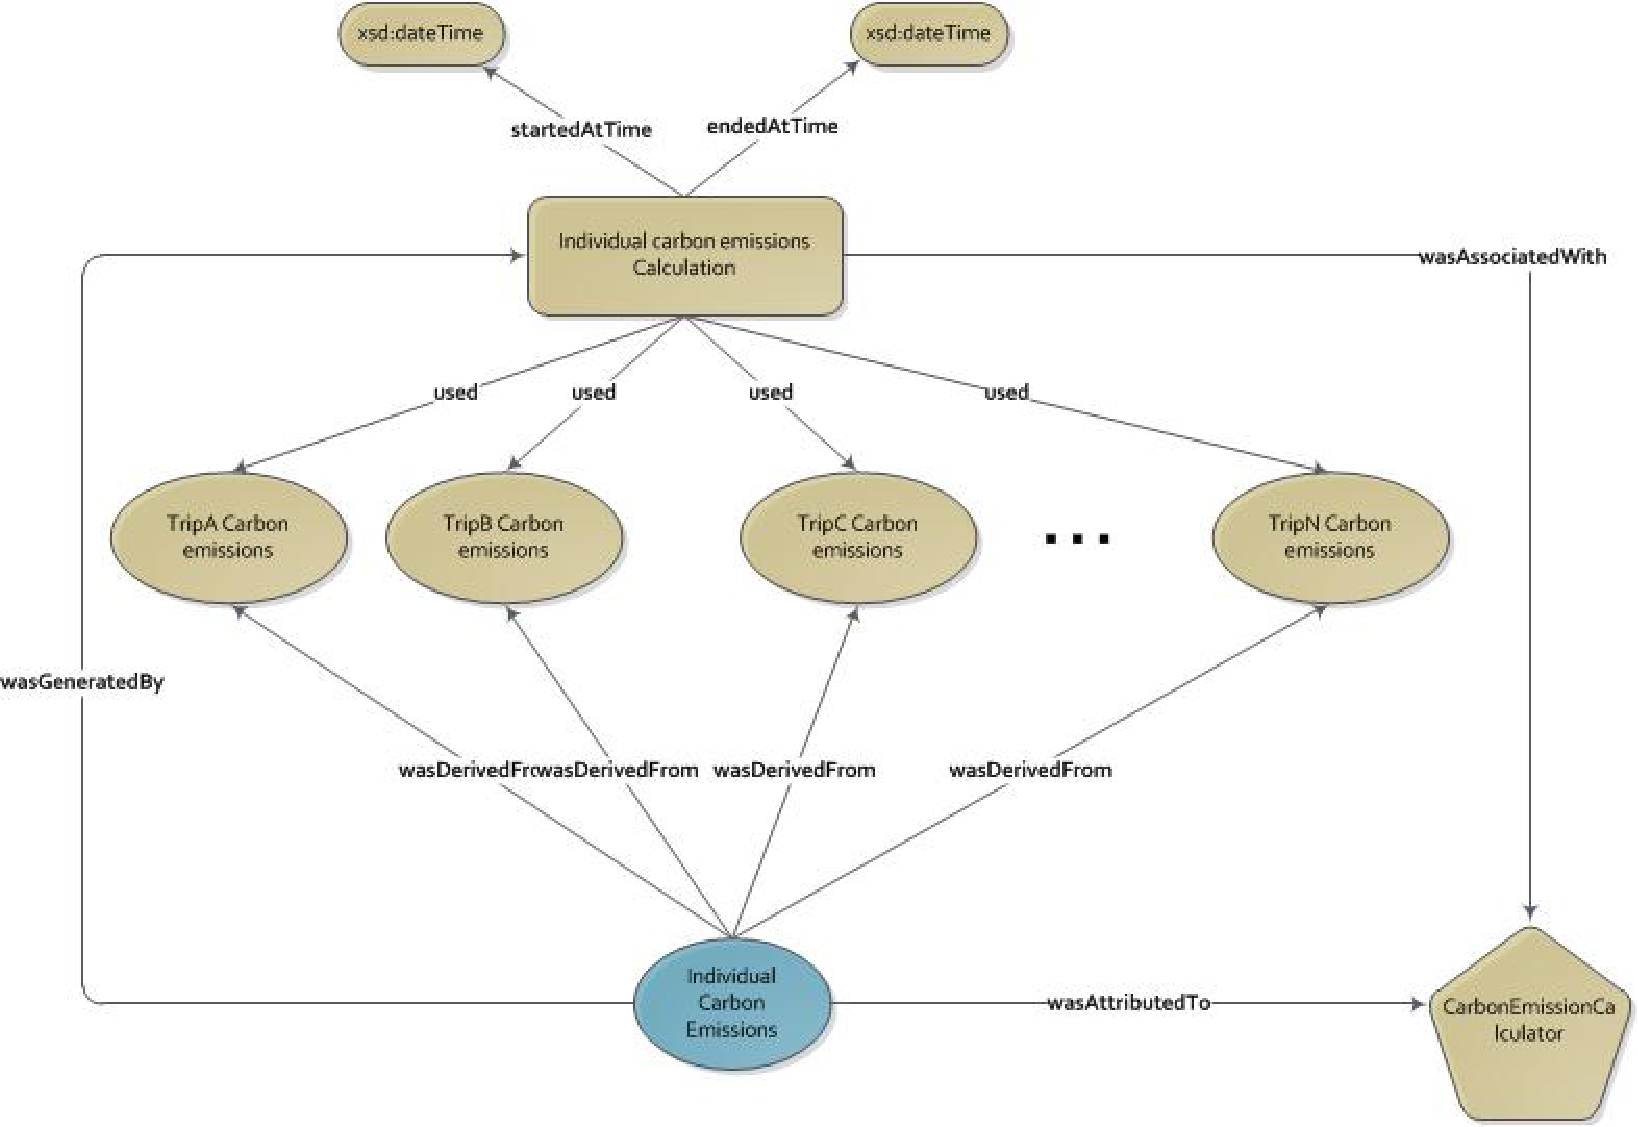
\includegraphics[scale=0.60]{./Figures/chapter3/figure5.pdf}
		\rule{35em}{0.5pt}
	\caption[Graph illustrating the provenance for individual carbon emissions]{Graph illustrating the provenance for individual carbon emissions}
	\label{fig:provIndividualCo2Graph}
\end{figure}

The same approach is adopted by the "Group Calculation" process, whereby the carbon emissions caused by all the trips made by all the members of the group in question are summed together. Figure \ref{fig:provGroupCo2Graph} illustrates the provenance graph for group carbon emissions.

\begin{figure}[htbp]
	\centering
		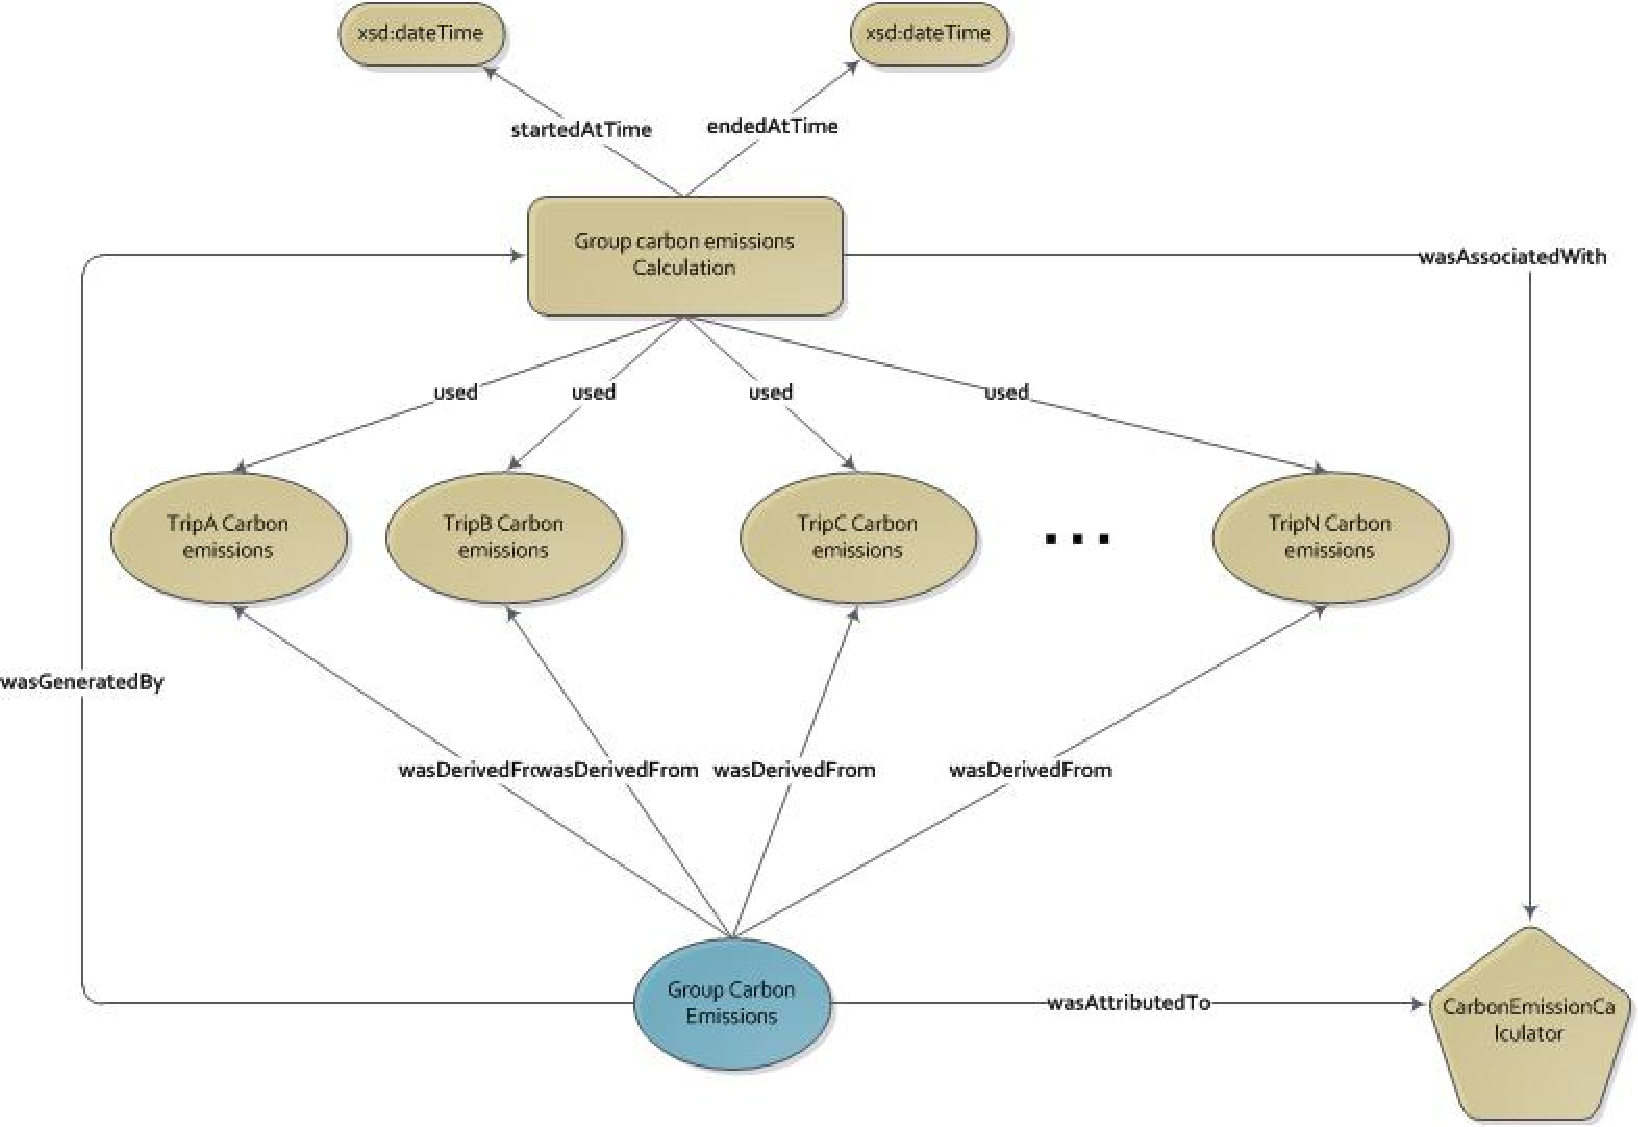
\includegraphics[scale=0.60]{./Figures/chapter3/figure6.pdf}
		\rule{35em}{0.5pt}
	\caption[Graph illustrating the provenance for group carbon emissions]{Graph illustrating the provenance for group carbon emissions}
	\label{fig:provGroupCo2Graph}
\end{figure}

\section{Storing Provenance}

The provenance graphs that we discussed earlier are represented in some application-specific format and stored in a relational database. More details about the process of creating and storing provenance graphs are presented in the next chapter.

\section{Fetching Provenance Information}

Our application has two options for viewing the provenance information for a specific piece of data; for instance, if users what to view provenance information in the form of graphs (like the above graphs), then a specific user interface can be used (next chapter describes this interface). Additionally, the application provides a REST web service that gets the identifier of a provenance graph and returns the graph in JSON format.

The JSON data below was returned after accessing the following service: http://127.0.0.1:8000/get-prov-graph/?provBundleId=1


\begin{verbatim}
{
   "wasDerivedFrom":{
      "_:id4":{
         "prov:usedEntity":"cf:tripLeg-2",
         "prov:generatedEntity":"cf:trip-1"
      },
      "_:id2":{
         "prov:usedEntity":"cf:tripLeg-1",
         "prov:generatedEntity":"cf:trip-1"
      }
   },
   "wasAssociatedWith":{
      "_:id6":{
         "prov:agent":"cf:ppoliani",
         "prov:activity":"cf:tripCreation"
      }
   },
   "wasAttributedTo":{
      "_:id7":{
         "prov:entity":"cf:trip-1",
         "prov:agent":"cf:ppoliani"
      }
   },
   "agent":{
      "cf:ppoliani":{
         "prov:type":"prov:Person",
         "foaf:mbox":"<mailto:ppoliani@gmail.com>"
      }
   },
   "entity":{
      "cf:tripLeg-1":{

      },
      "cf:trip-1":{

      },
      "cf:tripLeg-2":{

      }
   },
   "prefix":{
      "foaf":"http://xmlns.com/foaf/0.1/",
      "cf":"http://users.ecs.soton.ac.uk/pp6g11/ontology/carbonFooprints/"
   },
   "activity":{
      "cf:tripCreation":{

      }
   },
   "wasGeneratedBy":{
      "_:id5":{
         "prov:entity":"cf:trip-1",
         "prov:activity":"cf:tripCreation"
      },
      "_:id1":{
         "prov:entity":"cf:tripLeg-1",
         "prov:activity":"cf:tripCreation"
      },
      "_:id3":{
         "prov:entity":"cf:tripLeg-2",
         "prov:activity":"cf:tripCreation"
      }
   }
}

\end{verbatim}

Apparently, the above representation of provenance graphs is not for human consumption. It can rather be processed by a tool that is capable of reading and understanding this sort of serializations.

\section{Summary}

In this chapter we have described the benefits of adapting the provenance of electronic data technology in our application. We presented the processes during which the provenance information is captured and illustrated that information in the form of graphs. Finally, a very brief description about the storage and exposure of the captured provenance information was presented. We will come back to those issues in the following chapter. 